\documentclass[a4paper,12pt,twocolumn]{report}
\usepackage[utf8]{inputenc}
\usepackage{graphicx}
\usepackage{natbib}   % omit 'round' option if you prefer square brackets
\usepackage{hyperref}
\graphicspath{ {imgs/} }


%opening
\title{Effects of Swarming on Learning Rate of a Population}
\author{Dominic Hauton}



\begin{document}
\maketitle
\bibliographystyle{plainnat}

\section{Introduction}

The Upper Paleolithic (UP) transition shows evidence of rapid technological advancement. In this research we will attempt to reproduce \cite{powell2009late}'s findings on the advancement of knowledge during the UP transition using a modified version of \cite{henrich2004demography}'s transmission model. The aim is to explore the benefits of a more social population, simulated through an increased tendency for turtles to swarm.

If \cite{powell2009late}'s findings are correct, we should observe an increase in learning speed as turtles opt to socialize for a higher proportion of their time. We also hope to observe an exponential increase in learning as individuals start to require less resources and can therefore live in higher densities.

\section{Signaling}

We use \cite{henrich2004demography}'s work as a base for our signaling model. Turtles can misinterpret each other's foraging behavior, causing learning to have a chance of being detrimental. A 40\% chance of learning being beneficial to the learner is applied, making communication detrimental on average. As turtles learn from turtles with the highest level of knowledge in the area, given enough signaling, the mean knowledge level is expected to rise.

The turtles learn by observation, simulating copying foraging turtles in the vicinity. To prevent instant propagation of knowledge across the entire population, a turtle can only become as good as half the combined knowledge of itself and the teacher.

\section{Methodology}

Turtles are spawned in ten small colonies of fifty individuals with evenly distributed age and gamma distributed energy. The initial count and density is too high for the area so some turtles initially die due to overpopulation before a sustainable density is reached.

Swarming behavior is simulated through the turtle's movement. Turtles will forage for food until they gain a certain level of energy, at which point they will meander to the highest concentration of turtles within visible distance. This distance is higher than the signaling distance, so turtles benefit from wandering into a more populous area. This action carries a risk of turtles starving as it enters an overpopulated area.

This is a simplified version of the three-zones model used by \cite{1982simulation} and \cite{huth1992simulation}, to simulate schools of fish. We opt to ignore the average velocity of the turtles to prevent colonies moving, colliding and coalescing.

Throughout testing we vary the probability of a turtle meandering towards a more populated area, thereby simulating the willingness of an individual to socialize. In fig \ref{fig:swarming} the effect of probability can be observed to be working as intended.

We use \cite{edwards2007revisiting}'s gamma distributed movement distance to simulate movement per tick for each individual.

\begin{figure}[t]
 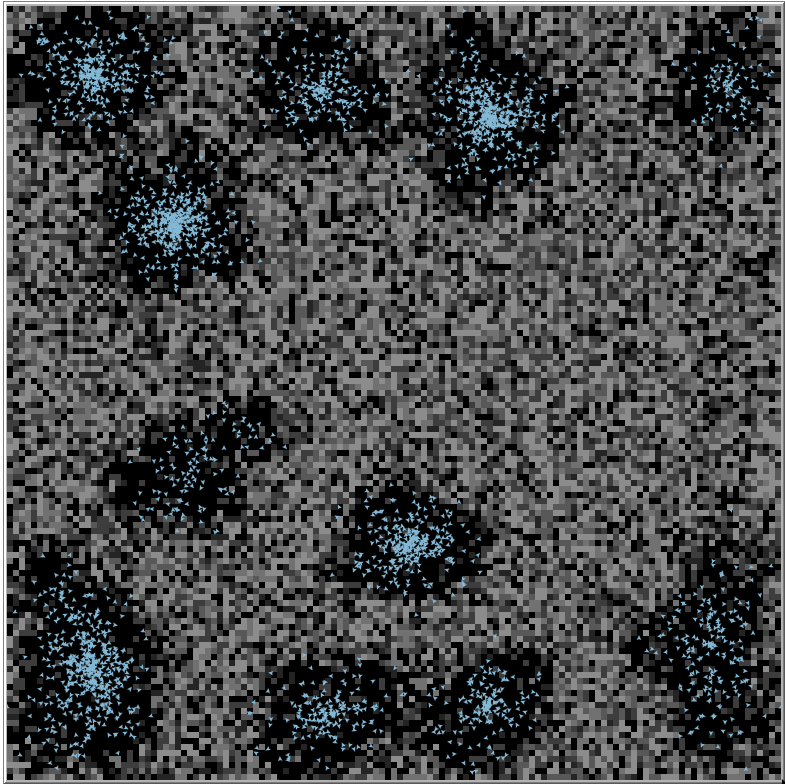
\includegraphics[width=0.24\textwidth]{swarming-high}
 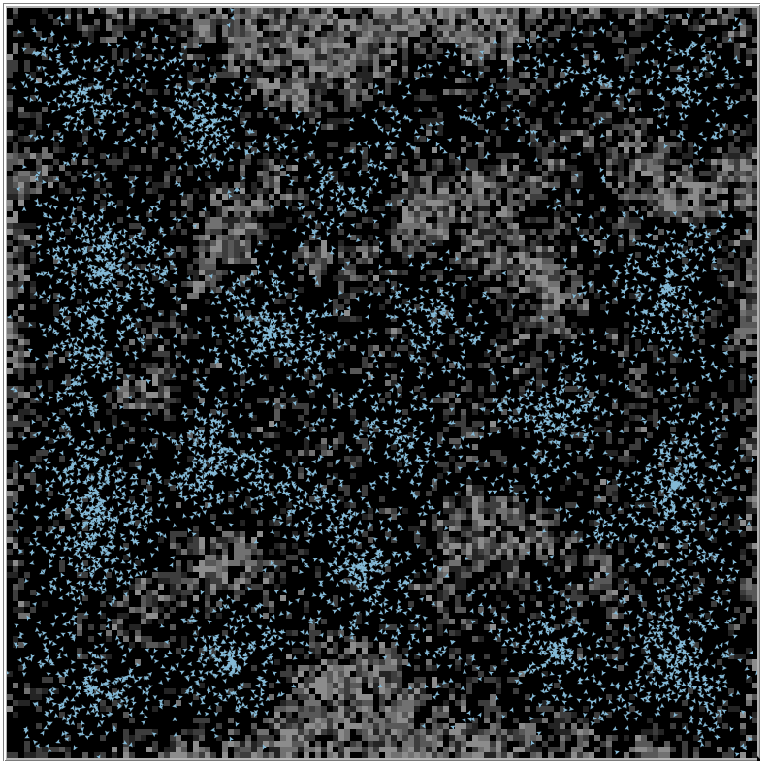
\includegraphics[width=0.24\textwidth]{swarming-low}
 \caption{Swarming Levels - 1.0 \& 0.8 resp.}
 \label{fig:swarming}
\end{figure}

The simulation is performed in Netlogo 6.0. The code is forked from a similar project by \cite{vcavce2007agent}. Fifty runs of simulation are performed for each of the tested swarming probabilities.

\section{Results}

The results of the simulation show an expected and statistically significant increase (using a p-value of 0.05) in knowledge progression within the population. Fig \ref{fig:table} shows a maximal knowledge progression occurring when turtles spent all of their free time in the swarm, only venturing out when hungry. There was no knowledge progression with a swarming rate of 0.7. Swarming values below 0.7 show no significant effects on learning, so we use 0.7 as our base reading.

\begin{figure}[b]
 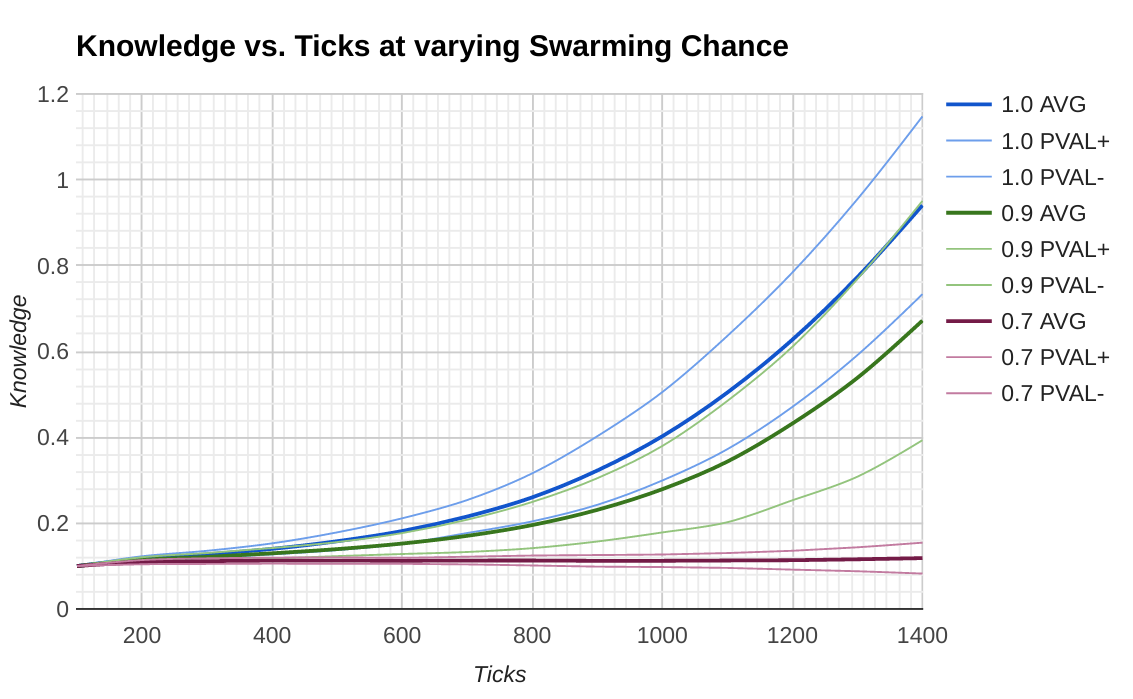
\includegraphics[width=0.5\textwidth]{swarming-effect}
 \caption{Knowledge vs Time - Results}
 \label{fig:table}
\end{figure}

An interesting observation is that fertile ground is required for swarming without the repulsion factor described by \cite{agueh2011analysis}.

When the food replacement rate is dropped past a critical point the swarming behavior leads to sudden death within the swarm as the members cannot get out of the highly populated area fast enough to eat. When the swarm dies the knowledge built up within it is lost.

\section{Conclusion}

We successfully managed to reproduce the increased rate of learning as population density is increased, demonstrated by \cite{powell2009late}. We have further shown that within a colony it is beneficial for members to spend as much time as possible in high density areas, as knowledge progression is accelerated.

The demise of a colony when the food replacement rate dropped may well be an explanation of sparks of intelligence observed during the UP transition, as described by \cite{powell2009late}. During prosperous times more social colonies excelled but as natural resources waned, those more social met their demise while less social, slower learners prevailed.

Although this work shows the benefits of a denser population it may be beneficial use a more complex swarming mechanism to see if similar results can be observed.

The model is also rather simple, with only one constant type of resource. It would be interesting to see colonies at 0.9 and 1.0 swarming probability cope with fluctuating food replacement rates, to see if the knowledge spikes in the UP transition can be reproduced. 

\bibliography{biblio1}

\end{document}
